\documentclass[11pt,letterpaper]{article}
\usepackage[utf8]{inputenc}

%----- Configuración del estilo del documento------%
\usepackage[table]{xcolor}
\usepackage{epsfig,graphicx}
\usepackage[left=2cm,right=2cm,top=1.8cm,bottom=2.3cm]{geometry}
\usepackage{fancyhdr}
\usepackage{lastpage}
\pagestyle{fancy}
\fancyhf{}
\rfoot{\textit{Página \thepage \hspace{1pt} de \pageref{LastPage}}}


%------ Paquetes matemáticos básicos --------%
\usepackage{amsmath}
\usepackage{amssymb}
\usepackage{amsthm}

%------ Texto aleatorio ----- %

\usepackage{lipsum}
\usepackage{enumitem}


\begin{document}

%------ Encabezado -------- %

\begin{center}
    \begin{minipage}{3cm}
    	\begin{center}
    		\includegraphics[height=3.4cm]{./imagenes/logo_unam.png}
    	\end{center}
    \end{minipage}\hfill
    \begin{minipage}{10cm}
    	\begin{center}
    	\textbf{\large Universidad Nacional Autónoma de México}\\[0.1cm]
        \textbf{Facultad de Ciencias}\\[0.1cm]
        \textbf{Matemáticas para las Ciencias Aplicadas $|$ Grupo 7048}\\[0.1cm]
        \textbf{Tarea 4 }\\[0.1cm]
        Real Araiza Yamile\\[0.1cm]
        Rodríguez López Luis Fernando\\[0.1cm]
        Tenorio Reyes Ihebel Luro\\[0.1cm]
        25/11/2024
    	\end{center}
    \end{minipage}\hfill
    \begin{minipage}{3cm}
    	\begin{center}
    		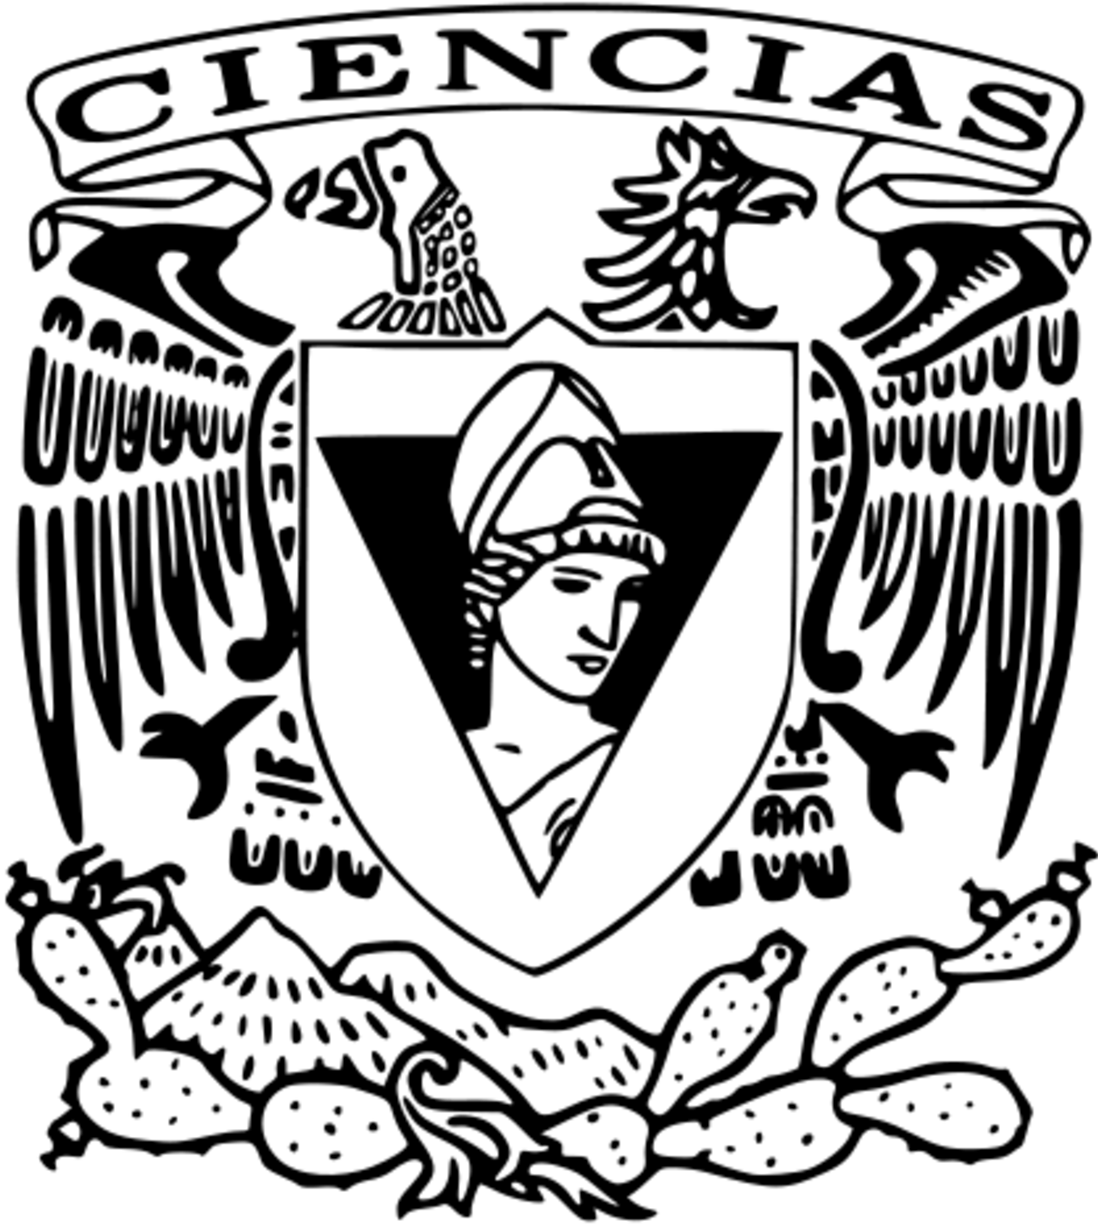
\includegraphics[height=3.4cm]{./imagenes/Logo_FC.png}
    	\end{center}
    \end{minipage}
\end{center}

\rule{17cm}{0.1mm}

%------ Fin de encabezado -------- %

%\section*{1ra Parte}

\subparagraph{Ejercicios: Review Exercises Capítulo 5 Anton-Bivens-Davis (pp. 408-412).}

% ---- 01. Ejercicio 13 IHEBEL ---- %
\section{Ejercicio 13, cap V Review Exercises.}
Evaluar la integral sustiyuyendo $u=x^2-1$
\begin{equation*}
  \int \frac{x}{(x^2-1)\sqrt{x^4-2x^2}}dx
\end{equation*}
Considerando:
\begin{equation*}
  \begin{split}
    u &= x^2-1\\
    u^2 &= x^4-2x^2+1\\
    du &= 2xdx\\
    dx &= \frac{du}{2x}
  \end{split}
\end{equation*}
Sustituyendo
\begin{equation*}
  \begin{split}
    \int \frac{x}{ (x^2-1) \sqrt{x^4-2x^2}} dx &= \int \frac{x\, du}{2x u \sqrt{u^2-1}} \\
    &= \frac{1}{2}\int \frac{du}{u\sqrt{u^2-1}} \\
    &= \frac{1}{2} \operatorname{sec}^{-1}\left(\frac{u}{1}\right) \quad \text{por fórmula 18} \\
    &= \frac{\operatorname{sec}^{-1}(u)}{2} \\
    &= \frac{\operatorname{arcsec}(x^2-1)}{2} + c
  \end{split}
\end{equation*}

% ---- 02. Ejercicio 23 YAMILE ---- %
\section{Ejercicio 23, cap V Review Exercises.}

% ---- 03. Ejercicio 42 YAMILE ---- %
\section{Ejercicio 42, cap V Review Exercises.}

% ---- 04. Ejercicio 53 LUIS ---- %
\section{Ejercicio 53, cap V Review Exercises.}

% ---- 05. Ejercicio 56 LUIS ---- %
\section{Ejercicio 56, cap V Review Exercises.}

% ---- 06. Ejercicio 64 LUIS ---- %
\section{Ejercicio 64, cap V Review Exercises.}

% ---- 07. Ejercicio 68 IHEBEL ---- %
\section{Ejercicio 68, cap V Review Exercises.}
Encuentra la función de posición de la particula que se mueve en el eje \textit{s}
\begin{equation*}
  \begin{split}
    a(t)=4cos(2t)\\
    v(0)=-1\\
    s(0)=-3
  \end{split}
\end{equation*}
Recordamos que la aceleracion es la derivada de la velocidad y la velocidad es la derivada de la posición.\\
Entonces...
\begin{equation*}
  v(t)=\int 4\cos(2t)dt = 4 \int \cos(2t)dt
\end{equation*}
considerando
\begin{equation*}
  \begin{split}
    u &= 2t\\
    du &= 2dt\\
    \frac{du}{2} &= dt
  \end{split}
\end{equation*}
Sustituyendo
\begin{equation*}
  \begin{split}
    4 \int \frac{\cos(u)du}{2} &= 2\int\cos(u)du\\
    &= 2\sin(u)\\
    &= 2\sin(2t)+c
  \end{split}
\end{equation*}
Esto es una familia de funciones, pero sabemos que $v(0)=-1$, entonces igualamos
\begin{equation*}
  \begin{split}
    2\sin(2(0))+c &= -1\\
    2\sin(0)+c &= -1\\
    c &= -1
  \end{split}
\end{equation*}
Por lo tanto
\begin{equation*}
  v(t)=2\sin(2t)-1
\end{equation*}
Ahora para obtener la funcion $s(t)$
\begin{equation*}
  \begin{split}
    s(t)&=\int (2\sin(2t)-1) dt\\
    &= \int 2\sin(2t)dt - \int dt\\
    &= 2\int\sin(2t)dt - t
  \end{split}
\end{equation*}
Consideramos
\begin{equation*}
  \begin{split}
    u &= 2t\\
    du &= 2dt\\
    \frac{du}{2} &= dt
  \end{split}
\end{equation*}
Sustituyendo
\begin{equation*}
  \begin{split}
    2\int \frac{\sin(u)du}{2}-t &= \int \sin(u)du + t\\
    &= -\cos(u)-t\\
    &= -\cos(2t)-t+c
  \end{split}
\end{equation*}
Caso similar al anterior, tenemos ahora una familia de funciones, pero sabemos que $s(0)=-3$, por lo tanto
\begin{equation*}
  \begin{split}
    -\cos(2(0))-(0)+c &= -3\\
    -\cos(0)+c &= -3\\
    -1+c &= -3 \\
    c &= -3 + 1\\
    c &= -2
  \end{split}
\end{equation*}
Por lo tanto, la ecuación de posición $s(t)$ está dada por
\begin{equation*}
  s(t)=-\cos(2t)-t-2
\end{equation*}

% ---- 08. Ejercicio 73 NADIE AUN ---- %
\section{Ejercicio 73, cap V Review Exercises.}

% ---- 09. Ejercicio 76 YAMILE ---- %
\section{Ejercicio 76, cap V Review Exercises.}

% ---- 10. Ejercicio 85 IHEBEL ---- %
\section{Ejercicio 85, cap V Review Exercises.}
Evaluar la integral por sustitución,
\begin{equation*}
  \int_0^1\sin^2(\pi x)\cos(\pi x)dx
\end{equation*}
Considerando:
\begin{equation*}
  \begin{split}
    u &= \sin(\pi x)\\
    du &= \cos(\pi x)\pi dx\\
    u^2 &= \sin^2(\pi x)\\
    u(0)&=\sin(\pi (0))=\sin(0)=0\\
    u(1) &= \sin(\pi (1)) = \sin(\pi))=0
  \end{split}
\end{equation*}
Sustituimos.
\begin{equation*}
  \pi \int_0^0u^2 \frac{\cos(\pi x)du}{\cos(2\pi)} = \pi \int_0^0 u^2du
\end{equation*}
Como el límite de integración superior es igual al inferior, el área bajo la curva dada es de 0.
\begin{equation*}
  \pi \int_0^0 u^2du = \pi (0) = 0
\end{equation*}
Por lo tanto, el valor de la integral es 0

%\section*{2da Parte}

\subparagraph{Ejercicios: Review Exercises Capítulo 6 Anton-Bivens-Davis (pp. 485-486).}

% ---- 11. Ejercicio 7 YAMILE ---- %
\section{Ejercicio 7, cap VI Review Exercises.}

% ---- 12. Ejercicio 13 LUIS ---- %
\section{Ejercicio 13, cap VI Review Exercises.}

% ---- 13. Ejercicio 16 YAMILE ---- %
\section{Ejercicio 16, cap VI Review Exercises.}

% ---- 14. Ejercicio 19 IHEBEL ---- %
\section{Ejercicio 19, cap VI Review Exercises.}
\textbf{a)} Un resorte ejerce una fuerza de 0.5N cuando es estirado más de su longitud natural.
Asumiendo que aplica la ley de Hooke, ¿cuánto trabajo fue efectuado al estar el resorte a esa longitud?\\
\textbf{b)} ¿Qué tanto trabajo más de su longitud natural se estiraría al aplicar 25J de trabajo?
\subsection*{a)}
Utilizaremos las formulas:\\
\begin{equation*}
  w=\int_{a}^{b}F(x)dx
\end{equation*}
\begin{equation*}
  \begin{split}
    F(x) &= kx\\
    \frac{F(x)}{x} &= k
  \end{split}
\end{equation*}
Primero calculamos la constante k
\begin{equation*}
  k=\frac{F(x)}{x}=\frac{0.5}{0.25}=2
\end{equation*}
de aquí $F(x)=2x$.\\
Ahora calculamos el trabajo.
\begin{equation*}
  \begin{split}
    w &= \int_{0}^{0.25}2xdx\\
    &= \left[ \frac{2}{2}x^2\right]^{0.25}_{0}\\
    &=(0.25)^2-(0)\\
    &=0.0625
  \end{split}
\end{equation*}
El trabajo realizado para estirar el resorte a 0.25m es 0.0675J.

\subsection*{b)}
Queremos calcular la distancia d, entonces, cambiamos la integral que sabemos que tiene un valor de 25J
\begin{equation*}
  \begin{split}
    \int_{0}^{d}2xdx &= 25\\
        [x^2]_{0}^{d} &=25\\
        (d)^2-(0)^2 &=25\\
        d^2 &=25\\
        d&=5
  \end{split}
\end{equation*}
Por lo tanto, la distancia es de 5 metros

\subparagraph{Ejercicios: Review Exercises Capítulo 7 Anton-Bivens-Davis (pp. 557-559).}

% ---- 15. Ejercicio 8 IHEBEL ---- %
\section{Ejercicio 8, cap VII Review Exercises.}
Evaluar la integral
\begin{equation*}
  \int_{0}^{1} \frac{x^3dx}{\sqrt{x^2+1}}
\end{equation*}
por:\\
\textit{a)} Integral por partes.\\
\textit{b)} Sustituyendo con $u=\sqrt{x^2+1}$.
\subsection*{a) Integral por partes}
Considerando
\begin{equation*}
  \begin{split}
    u &= x^2\\
    du &= 2xdx\\
    \\
    dv &= x(x^2+1)^{-{\frac{1}{2}}}\\
    v &= \int \frac{x}{\sqrt{x^2+1}}dx
  \end{split}
\end{equation*}
consideramos
\begin{equation*}
  \begin{split}
    a &= x^2+1\\
    da &= 2xdx\\
    \frac{da}{2x} &= dx
  \end{split}
\end{equation*}
\begin{equation*}
  \begin{split}
    v &= \int \frac{xda}{2x\sqrt{a}}\\
    &= \frac{1}{2} \int \frac{da}{\sqrt{a}}\\
    &= a^{\frac{1}{2}}\\
    &= \sqrt{x^2=1}
  \end{split}
\end{equation*}
Sustiuyendo usando la formula de integracion por partes
\begin{equation*}
  \int u dv = uv - \int v du
\end{equation*}
Tenemos
\begin{equation*}
    \int \frac{xx^2}{\sqrt{x^2+1}}dx=x^2\sqrt{x^2+1}-\int\sqrt{x^2+1}2xdx
\end{equation*}
Aplicamos sustitución considerando
\begin{equation*}
  \begin{split}
    a &= x^2+1\\
    da &= 2xdx\\
    \frac{da}{2x} &= dx
  \end{split}
\end{equation*}
\begin{equation*}
  \begin{split}
    \int\frac{\sqrt{a}2xda}{2x} &= \int \sqrt{a}da\\
    &=\frac{2}{3}a^{\frac{3}{2}}\\
    &=\frac{2}{3}(x^2+1)^{\frac{3}{2}}+c
  \end{split}
\end{equation*}
Ahora evaluamos en los limites dados
\begin{equation*}
  \begin{split}
    \int_{0}^{1}\frac{x^3}{\sqrt{x^2+1}} &= \left[ x^2\sqrt{x^2+1}-\frac{2}{3}(x^2+1)^{\frac{3}{2}}\right]^{1}_{0}\\
    &=\left((1)^2\sqrt{(1)^2+1}-\frac{2}{3}((1)^2+1)^{\frac{3}{2}}\right) - \left(\underbrace{(0)^2\sqrt{(0)^2+1}}_{0}-\frac{2}{3}\underbrace{((0)^2+1)^{\frac{3}{2}}}_{1}\right)\\
    &=2^{\frac{1}{2}}-\frac{2}{3}(2)^{\frac{3}{2}}+\frac{2}{3}\\
    &=2^{\frac{1}{2}}(1-\frac{2}{3}(2))+\frac{2}{3}\\
    &=2^{\frac{1}{2}}(\frac{3}{3}-\frac{4}{3})+\frac{2}{3}\\
    &=2^{\frac{1}{2}}(-\frac{1}{3})+\frac{2}{3}\\
    &=\frac{2}{3}-\frac{\sqrt{2}}{3}\\
    &=\frac{2-\sqrt{2}}{3}
  \end{split}
\end{equation*}

\subsection*{b) Sustitucion}
Consideramos
\begin{equation*}
  \begin{split}
    u &= \sqrt{x^2+1} =(x^2+1)^{\frac{1}{2}}\\
    du &= \frac{1}{2}(x^2+1)^{-\frac{1}{2}}2xdx\\
    \frac{\sqrt{x^2+1}du}{x} &= dx\\
    u^2 &= x^2+1\\
    u^2-1 &= x^2\\
    \\
    u(1) &= \sqrt{(1)^2+1} = \sqrt{2} = (2)^{\frac{1}{2}}\\
    u(0) &= \sqrt{(0)^2+1} = 1
  \end{split}
\end{equation*}
Sustituimos
\begin{equation*}
  \begin{split}
    \int_{0}^{1} \frac{x^3}{\sqrt{x^2+1}}dx &= \int_{1}^{\sqrt{2}} \frac{x(u^2-1)\sqrt{x^2+1}du}{x\sqrt{x^2+1}}\\
    &= \int_{1}^{\sqrt{2}}(u^2-1)du\\
    &= \left( \frac{1}{3}(2^{\frac{1}{2}})^3-2^{\frac{1}{2}} \right) - \left( \frac{1}{3}(1)^{\frac{1}{2}}-1 \right)\\
    &=2^{\frac{1}{2}}\left( \frac{2}{3}-\frac{3}{3} \right)+\frac{2}{3}\\
    &=2^{\frac{1}{2}}\left( -\frac{1}{3}\right) + \frac{2}{3}\\
    &=-\frac{\sqrt{2}}{3}+\frac{2}{3}\\
    &=\frac{2-\sqrt{2}}{3}
  \end{split}
\end{equation*}
En ambos casos obtenemos el mismo resultado.

% ---- 16. Ejercicio 14 LUIS ---- %
\section{Ejercicio 14, cap VII Review Exercises.}

% ---- 17. Ejercicio 33 LUIS ---- %
\section{Ejercicio 33, cap VII Review Exercises.}

% ---- 18. Ejercicio 41 IHEBEL ---- %
\section{Ejercicio 41, cap VII Review Exercises.}
Aproxima la integral
\begin{equation*}
  \int_1^3 \frac{1}{\sqrt{x+1}}dx
\end{equation*}
usando...\\
\textbf{a)} Aproximacion del punto medio $M_{10}$.\\
\textbf{b)} Aproximacion trapezoidal $T_{10}$.\\
\textbf{c)} Regla de Simpson para la aproximacion $S_{20}$.\\
En cada caso, encontrar el error absoluto.\\
Considerar al menos 5 décimas.
\subsection*{Valor real}
\begin{equation*}
  \begin{split}
    u &= x+1\\
    du &= dx\\
    u(1) &= (1)+1 = 2\\
    u(3) &= (3)+1 = 4 
  \end{split}
\end{equation*}
\begin{equation*}
  \begin{split}
    \int_1^3 \frac{1}{\sqrt{x+1}}dx &= \int_2^4 u^{-\frac{1}{2}}\\
    &=\left[ 2u^{\frac{1}{2}} \right]_2^4\\
    &=2\sqrt{4}-2\sqrt{2}\\
    &=2(2)-2\sqrt{2}\\
    &=4-2\sqrt{2}\\
    &\approx 1.17157 \ \text{con calculadora}
  \end{split}
  \end{equation*}
El valor real de la funcion $V_R$ es de 1.17157u.
  

\subsection*{a) Punto Medio $M_{10}$}
\begin{equation*}
  \int_a^b f(x)dx=\left( \frac{b-a}{n}\right)\left( y_{m_1}+y_{m_2}+...+y_{m_n}\right)
\end{equation*}
Tenemos que
\begin{equation*}
  \begin{split}
    \Delta x &= \left( \frac{b-a}{n} \right)\\
    x_i &= a+(i-(\frac{1}{2}))\Delta x
  \end{split}
\end{equation*}
Sustituyendo e interpretando la serie y.
\begin{equation*}
    \int_a^b f(x)dx = \frac{b-a}{n}\sum_{i=1}^n\left(f\left( a+(i-\frac{1}{2})(\frac{b-a}{n}) \right)\right)
\end{equation*}
Calculamos la diferencial de x
\begin{equation*}
  \Delta x = \frac{b-a}{n} = \frac{3-1}{10}+\frac{2}{10}=\frac{1}{5}
\end{equation*}
susituyendo, obtenemos la aproximación:
\begin{equation*}
  \begin{split}
    \int_1^3 \frac{1}{\sqrt{x+1}}dx &\approx \frac{1}{5}\sum_{i=1}^{10}\frac{1}{\sqrt{(1+(i-\frac{1}{2})(\frac{1}{5}))+1}}\\
    &\approx \frac{1}{5}\sum_{i=1}^{10}\frac{1}{\sqrt{\frac{1}{5}}(i-\frac{i}{2})}\\
    &\approx 1.17138 \ \ \text{Resolviendo con calculadora}
  \end{split}
\end{equation*}
El error es
\begin{equation*}
    E_A=\|V_R-T_{10} \|=1.9x10^{-4}
\end{equation*}
El valor de la aproximación es de 1.17138u con un error de $1.9x10^{-4}$


\subsection*{b) Trapezoidal $T_{10}$}
Tenemos primero que
\begin{equation*}
  \int_a^b f(x)dx=\left( \frac{b-a}{2n}\right)\left( y_0+2y_1+2y_2y+2+...+2y_{n-1}+y_n\right)
\end{equation*}
Luego, tenemos que
\begin{equation*}
  \begin{split}
    x_i &= a+i\Delta x\\
    y_i &= f(x_i)
  \end{split}
\end{equation*}
Entonces
\begin{equation*}
  \begin{split}
    \int_a^b f(x)dx &= \left( \frac{b-a}{2n}\right)\left( y_0+2y_1+2y_2y+2+...+2y_{n-1}+y_n\right)\\
    &=\left( \frac{\Delta x}{2}\right)\left( y_0+y_n+2y_1+2y_2y+2+...+2y_{n-1}\right)\\
    &=\left( \frac{\Delta x}{2}\right)\left( y_0+y_n+2\sum_{i=0}^{n-1}y_i \right)\\
    &=\left( \frac{\Delta x}{2}\right)\left( f(a)+f(b)+2\sum_{i=0}^{n-1}f(a+i\Delta x) \right)
  \end{split}
\end{equation*}
Sustituyendo para obtener la aproximación
\begin{equation*}
  \begin{split}
    \int_1^3 \frac{1}{\sqrt{x+1}}dx &\approx \frac{1}{10}\left( \frac{1}{\sqrt{2}}+\frac{1}{2}=2\sum_{i=1}^{9}\frac{1}{\sqrt{(1+\frac{x}{5})+1}} \right)\\
    &\approx 1.17195 \ \ \text{Evaluando con calculadora}
  \end{split}
\end{equation*}
El error es
\begin{equation*}
    E_A=\|V_R-T_{10} \|=3.8x10^{-4}.
\end{equation*}
El valor aproximado de la función es de 1.17195u con un error de $3.8x10^{-4}$

\subsection*{c) Regla de Simpson}
\begin{equation*}
  \begin{split}
    \int_a^b f(x)dx &= \frac{1}{3}\left( 2M_k+T_k \right)\\
    S_n = \frac{1}{3}\left( 2M_{\frac{n}{2}}+T_{\frac{n}{2}}  \right)
    \end{split}
\end{equation*}
Por lo tanto, la aproximación por regla de Simpson esta dada por
\begin{equation*}
  S_{20}\approx\frac{1}{3}\left( 2\underbrace{M_{10}}_{\text{a)}}+\underbrace{T_{10}}_{\text{b)}}\right)\approx 1.17187.
\end{equation*}

\begin{equation*}
    E_A=\|V_R-S_{20} \|=0
\end{equation*}
Con la regla de Simpson, la aproximacion es de 1.17187u, que es igual al valor real (considerando solo 5 décimas)

% ---- 19. Ejercicio 51 YAMILE ---- %
\section{Ejercicio 51, cap VII Review Exercises.}


% ---- 20. Ejercicio NADIE AUN ---- %
\section{Ejercicio: Classroom.}

\end{document}
